\section{Transfer Learning}

Transfer Learning is a technique used to train machine learning models that is particularly popular for the task of image classification. Transfer Learning utilizes models that have been previously trained for related (usually broader and more diverse) tasks and leverages their knowledge as a starting point for training a new model for the current, more specific task. The intuition behind this technique is simple, as it is plainly evident that much of the knowledge required to identify motor-vehicles (a broader problem) can be reused to identify cars (a related, more specific problem).

Transfer Learning was first outlined as a technique in 1976 by Bozinovski and Fulgosi  \cite{16}, and has been noted in recent times to outperform other state-of-the-art methods. This, in conjunction with the increasing accessibility of high-quality pre-trained models (ResNet, NASNet, MobileNet, etc.) has made it popular as one of the go-to techniques for machine learning problems, especially so in the field of computer vision.

The transfer learning process is largely divided into three parts: pre-training, feature extraction and fine-tuning. During pre-training, a model is trained using a very large and generic dataset, allowing it to learn general representations that are likely to be useful across multiple diverse and more specific tasks. An example of this is the ImageNet project, a large database of over 14 million generic images belonging to over 20,000 categories. Multiple pre-trained models are trained on the ImageNet database (again, ResNet, NASNet, MobileNet, etc.) as the feature representations learned from this database are general and therefore applicable to most image-classification tasks.  

The weights of the models trained on these large datasets are then saved and can be used as starting points for new models oriented towards more specific problems. 

Feature extraction then leverages the previously learned representations of the pre-trained models by removing the existing classifier (for the broader problem) and replacing it with a new classifier on top of the rest of the existing model, which is subsequently trained from scratch using the dataset for the new, more specific task. In this process, only the weights of the newly added classifier are modified. The base CNN already contains feature representations that are to be leveraged, and therefore remains frozen i.e. its weights are not updated.

As such, the base CNN contains features that are generically useful while the final classifier contains features that are specifically useful to the current classification task. Finally, fine-tuning takes the now modified pre-trained model and makes it as specific as possible by unfreezing some of the top layers of the base CNN and re-training the model for a set amount of time. Via this process, the higher-order feature representations of the base CNN model can be subtly modified (or fine-tuned) to specifically suit the current classification problem. 

Transfer learning is beneficial and preferred for multiple reasons. Firstly, it reduces the need for extensive amounts of training data, which is often simply infeasible and/or too expensive and time-consuming to obtain. This allows for high-quality models to be trained for problems that might otherwise suffer from a lower availability of good data. Secondly, the use of transfer learning also greatly hastens the process of training. In the absence of transfer learning, large models have to be trained entirely from scratch, a process which can be extremely time-intensive even with the smallest datasets. With transfer learning, one only needs to train a classifier on top of existing models thereby reducing the amount of computation required by several magnitudes, allowing for models with far better performance to be trained in far less time. Lastly, transfer learning makes the process of training ML models more accessible given the relative ease of training complex models with this technique, allowing for a larger number of individuals with fewer resources to put their models into practice. 

\section{Pre-Trained CNNs}
Since the advent of AlexNet  \cite{17}, multiple deep CNNs have been developed for a variety of image classification tasks. The architecture of these models has become increasingly deeper and more complex, and consequently their performance has simultaneously gotten better. There have also been multiple innovations in the architecture of these networks that have resulted in faster and better performing networks over time. With the advent of the previously mentioned ImageNet project, pre-trained models using the ImageNet database as a starting training point have advanced various image-related tasks such as classification, segmentation and object detection rapidly. We further briefly discuss some of the pre-trained networks we used.

\subsection{ResNet}
ResNet(s)  \cite{18}  \cite{19} (short for a Residual Network) are a class of various pre-trained CNNs (ResNet50, ResNet50V2, ResNet152V2, etc.) that utilize skip-connections to solve the problem of a vanishing gradient. The ResNet architecture does this through the introduction of a residual block, simply introducing an intermediate skipped input to the output of a series of convolutional blocks. This technique smooths the gradient during the training process, allowing a solution to a vanishing gradient. Empirically, these networks have been found to be much easier to optimize and show considerable gains in accuracy as compared to other deep CNNs.
\begin{center}
   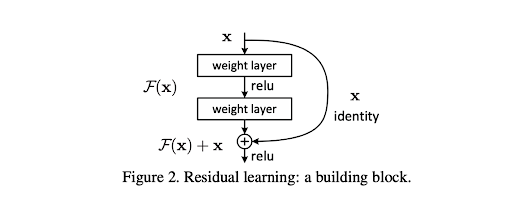
\includegraphics[width=5in]{images/3.1.png} 
   \\\fontsize{11pt}{24pt} Figure 3.1: A residual block.
\end{center}
				

\subsection{MobileNet}
MobileNet is CNN proposed by Howard et al.  \cite{20} that uses depth-wise separable convolutions to design relatively lightweight networks primarily aimed at having smaller sizes while maintaining parity in performance to larger, state-of-the-art models. The primary innovation of MobileNet is a depth-wise separable convolution, which differs from the 2D convolution generally used in other CNNs. 2D convolutions are performed over multiple/all input channels of an image (R,G and B, for example). In depth-wise convolutions, each channel is kept separate and is convolved independently. The output obtained from each channel is stacked together to get the output as a multi-dimensional tensor. Finally then, these output channels are combined to form a set number of channels, adding the separable part to the depth-wise convolution. This process is far more efficient as it requires a far lesser amount of mathematical computation than a regular 2D convolution resulting in faster networks with fewer parameters. 



   








\begin{center}
   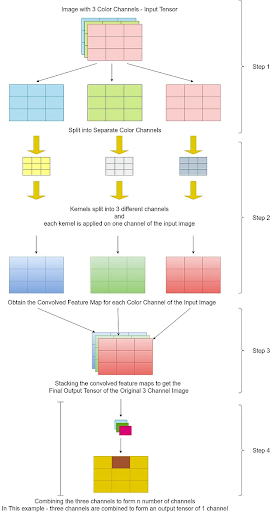
\includegraphics[width=4.5in]{images/3.2.png} 
   \\\fontsize{11pt}{24pt} Figure 3.2: MobileNet convolution.
\end{center}



 


\subsection{DenseNet}
DenseNet (short for a Densely Connected Network), is a CNN proposed by Huang et al.  \cite{21} that uses densely connected layers to pass the feature map of a specific layer to all subsequent layers in the network. The aim of DenseNet was to alleviate the vanishing gradient problem and to strengthen feature propagation via the densely connected layers. DenseNets also require fewer parameters. As each layer receives the output (and representations) of all previous layers, networks can be more compact and can contain fewer channels, allowing for higher size and memory efficiency. DenseNets have been shown to achieve state-of-the-art results on many image-classification problems. 


\begin{center}
   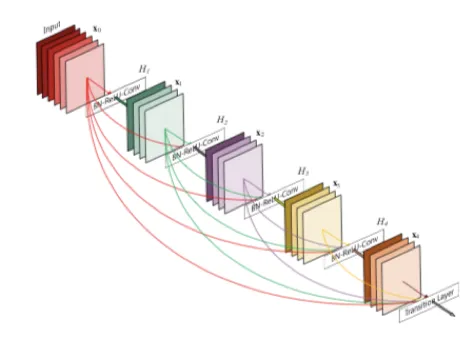
\includegraphics[width=6in]{images/3.3.png} 
   \\\fontsize{11pt}{24pt} Figure 3.3: DenseNet
\end{center}

				
\section{Metaheuristic Algorithms}
Metaheuristic algorithms are techniques for solving optimization problems that are computationally expensive to solve optimally. They aim to generate satisfactorily good solutions that are ideally near-optimal, and are important in problems where the solution space is extremely large and/or requires an inordinate amount of resources in terms of time and computational power to properly solve. These algorithms are stochastic and often contain a degree of randomness in generating new solutions. These algorithms have been of specific research interest because of their ability to avoid early convergence and because of their flexibility in being easily modifiable and applicable to almost any arbitrary optimization problem. These algorithms have been successfully used in various engineering fields such as Power, Infrastructure/Civil Engineering and Communication. 

Metaheuristic algorithms find inspiration from various natural phenomena, and can broadly be classified as following on the basis of their behavior:
Evolutionary Algorithms: Based on genetic evolution in nature, these algorithms involve populations of solutions that are iteratively combined together according to defined procedures to generate newer populations of solutions. The first and most popular algorithm of this sort is the Genetic Algorithm  \cite{9}, based on classical Darwinian evolution. 
Swarm-based Algorithms: These algorithms find their inspiration in the collective large-scale group behavior of natural beings, aiming to mimic their interactions in exploring a solution space for a particular problem. The most popular algorithm of this sort is Particle Swarm Optimization  \cite{10}, based on the behavior of birds. 
Physics-based Algorithms: These algorithms mimic physical phenomena such as gravity to find optimal solutions to a search space. An example is Simulated Annealing  \cite{22}. 
Human-based Algorithms: Similar to swarm-based algorithms, these algorithms are based on the group behaviors of human beings. An example is TLBO  \cite{23}.  

We further discuss some of the algorithms we chose to use for our work.
\subsection{Particle Swarm Optimization}
Particle Swarm Optimization  \cite{10} is a swarm-based metaheuristic algorithm based on the group behavior of birds that was introduced by Kennedy and Eberheart in 1995. This algorithm was theorized on the basis of socio-biological research, which believes that a school of fish/a flock of birds exhibit group movement that benefits from the knowledge of all members in the group. Mimicking this behavior in a solution space can thus lead to close-to-optimal satisfactory solutions for complex optimization problems. 

The algorithm begins with P particles denoting P distinct solutions, with each particle having at any iteration t a position Xi(t) and a velocity Vi(t). Per iteration, the position and velocity of each particle are updated according to the equations (3.1) and (3.2):\\ 
Xi(t + 1) = Xi(t) + Vi(t)          – (3.1)\\ 
Vi(t + 1) = w.Vi(t) + c1.r1.(pbest(i) - Xi(tt)) + c2.r2.(gbest - Xi(t))     - (3.2)\\
where r1 and r2 are random numbers between 0 and 1, c1 and c2 are parameters of the algorithms, \\
pbest(i) is the best position of particle i thus far \\
and gbest is the best solution found thus far. \\
Both subtractions in equation (3.2) are vector subtractions. 


The parameter w is called the inertia weight constant and is between 0 and 1, determining to what extent the new velocity of a particle is dependent upon its previous velocity. The parameters c1 and c2 are respectively called the cognitive and social constants, and denote the weightage given to local and global knowledge in affecting the change in velocity.

\begin{center}
   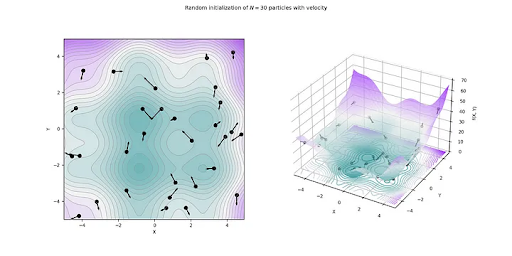
\includegraphics[width=5.5in]{images/3.4.png} 
   \\\fontsize{11pt}{24pt} Figure 3.4: Visualization of PSO
\end{center}



A modified version of PSO called Hierarchical PSO with Time Varying Acceleration Constants (HPSO-TVAC) was introduced by Ghasemi et al.  \cite{24} in  2017.
\subsection{Genetic Algorithm}
The Genetic Algorithm  \cite{9} is an evolutionary metaheuristic algorithm first developed in the 1960s. It mimics darwinian evolution and involves a population of individuals (or solutions), each represented by a certain chromosome consisting of various genes. The fitness (or the objective function that we’d like to optimize) is measured for each individual, and the fittest individuals in the population then ‘reproduce’ to generate new individuals for the next iteration using a process called crossover. To mimic natural evolution, these new individuals can also have random changes via the process of mutation. 


\begin{center}
   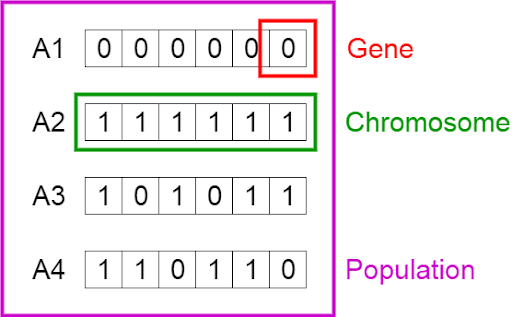
\includegraphics[width=5in]{images/3.5.png} 
   \\\fontsize{11pt}{24pt} Figure 3.5: Genetic Algorithm Representation
\end{center}
			


\begin{center}
   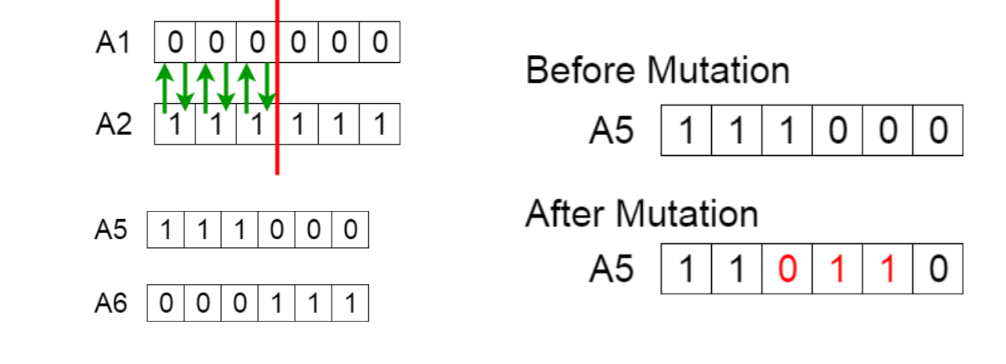
\includegraphics[width=5in]{images/3.6.png} 
   \\\fontsize{11pt}{24pt} Figure 3.6: Crossover and Mutation
\end{center}


We also use several other metaheuristics such as Coral Reef Optimization  \cite{26}. Grey Wolf Optimization  \cite{12} and Harmony Search  \cite{27}.
\section{Feature Selection}
Often, all features of a given dataset are not relevant to the machine learning problem at hand. In these cases, Feature Selection refers to the task of removing the best features from a dataset to increase performance of the model being built. Feature Selection is a critical process in machine learning that is specifically important with data where there exist a significantly large number of features. In such cases, learning often causes overfitting which in turn causes worse generalization and thus worse real-world performance of the model. In these cases, Feature Selection is desirable as it not only increases performance but also decreases computational complexity. Feature selection can be particularly important in the task of image classification. CNNs output feature representations that are significantly large in nature. Often, not all of the features in an image are important to the classification task at hand. For example, in the particular field of AI-generated image detection, AI-generated images have certain marked characteristics that can be more important to the classification task than other more generic features. For instance, AI-generated images often have issues with fingers when generating human portraits, as shown in figure 3.7. In these cases, feature selection can help identify and focus on these aspects of AI-images resulting in better classification accuracy.


\begin{center}
   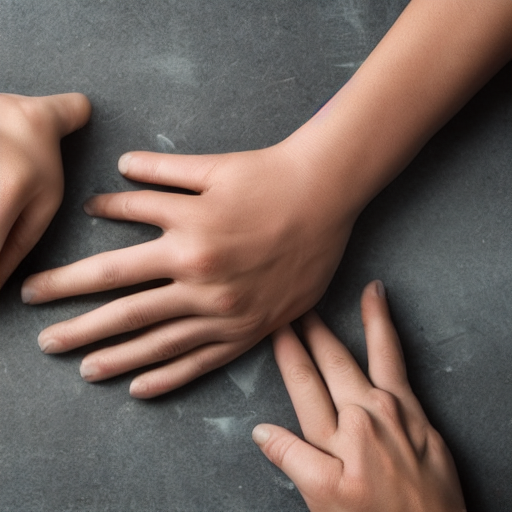
\includegraphics[width=3in]{images/3.7.png} 
   \\\fontsize{11pt}{24pt} Figure 3.7: an AI-generated image of a hand.
\end{center}



Generally, the techniques are classified into three categories: filter, wrapper and embedded methods. Filter methods are independent of the learning algorithm, while Wrapper methods include learning algorithms and train a new model for every feature subset selected. Embedded methods usually consist of some combination of filter and wrapper methods. One of the many wrapper methods is a metaheuristic algorithm, having a long history of being used for this specific application  \cite{13}. 
